\documentclass[11pt, leqno]{scrartcl}
\usepackage{polski}
\usepackage[polish]{babel}

\usepackage{graphicx, float, caption, subcaption}
\usepackage{tabularx, multirow, hyperref, enumitem}
\usepackage{listings, xcolor}
\usepackage{amsmath, amssymb}
\usepackage{algorithm}
\usepackage{algpseudocode}
%\usepackage{minted}

\hypersetup{
    colorlinks=true,
    linkcolor=black,
    urlcolor=black,
    citecolor=black
}

\definecolor{md-black}{rgb}{0.12, 0.12, 0.12}
\definecolor{md-teal}{rgb}{0.38, 0.79, 0.69}
\definecolor{md-mauve}{rgb}{0.76, 0.52, 0.75}
\definecolor{md-yellow}{rgb}{0.86, 0.86, 0.67}
\definecolor{md-green}{rgb}{0.13, 0.55, 0.13}
\definecolor{md-red}{rgb}{0.82, 0.10, 0.14}
\definecolor{md-purple}{rgb}{0.69, 0.33, 0.73}
\definecolor{md-orange}{rgb}{0.96, 0.42, 0.18}
\definecolor{md-gray}{rgb}{0.44, 0.46, 0.51}
\lstset{
    language=Python,
    basicstyle=\color{md-teal}\ttfamily,
    keywordstyle=\color{md-mauve},
    commentstyle=\color{md-green},
    stringstyle=\color{md-red},
    numbers=left,
    numberstyle=\small\color{md-gray}\ttfamily,
    stepnumber=1,
    numbersep=5pt,
    backgroundcolor=\color{md-black},
    showspaces=false,
    showstringspaces=false,
    showtabs=false,
    frame=none,
    tabsize=4,
    captionpos=b,
    breaklines=true,
    breakatwhitespace=false,
    escapeinside={\%*}{*)},
    numbersep=-10pt,
    morekeywords={as},
    classoffset=1,
    morekeywords={quad, quad_vec, trapz, simps, linregress,
        newton},
    keywordstyle=\color{md-yellow},
    classoffset=0
}

\graphicspath{{../images/}}

\title{I zestaw zadań - Mnożenie macierzy}
\author{Kacper Kozubowski, Mateusz Podmokły \\ III
    rok Informatyka WI}
\date{2 październik 2024}

\begin{document}
    \maketitle
    \section{Treść zadania}
    Należy wygenerować macierze losowe o wartościach
    z przedziału otwartego $(10^{-8},1.0)$
    i zaimplementować
    \begin{enumerate}
        \item Rekurencyjne mnożenie macierzy metodą Binét'a
        \item Rekurencyjne mnożenie macierzy metodą Strassena
        \item Mnożenie macierzy metodą AI na podstawie
            artykułu w Nature
    \end{enumerate}
    Proszę zliczać liczbę operacji zmienno-przecinkowych
    wykonywanych podczas mnożenia macierzy.

    \section{Specyfikacja użytego środowiska}
    Specyfikacja:
    \begin{itemize}
        \item Środowisko: Jupyter Notebook,
        \item Język programowania: Python,
        \item System operacyjny: Microsoft Windows 11,
        \item Architektura systemu: x64.
    \end{itemize}

    \section{Działanie algorytmów}
    \subsection{Wykorzystane biblioteki}
    W realizacji rozwiązania wykorzystane zostały następujące
    biblioteki:
    \begin{lstlisting}
    import numpy as np
    import matplotlib.pyplot as plt
    import time
    \end{lstlisting}
    \subsection{Pseudokod}
    \begin{algorithm}[H]
        \caption{Algorytm Binét'a}
        \begin{algorithmic}
            \State \textbf{Input:} A, B
            \State \textbf{Output:} C
            \Function{binet}{A, B}
                \State n = size(A)
                \If{n = 1}
                    \State return A * B
                \EndIf
                \State
                \State mid = n \textbf{div} 2
                \State A11 = A[1:n, 1:n]       // Górny lewy blok
                \State A12 = A[1:n, n+1:2n]    // Górny prawy blok
                \State A21 = A[n+1:2n, 1:n]    // Dolny lewy blok
                \State A22 = A[n+1:2n, n+1:2n] // Dolny prawy blok
                \State B11 = B[1:n, 1:n]
                \State B12 = B[1:n, n+1:2n]
                \State B21 = B[n+1:2n, 1:n]
                \State B22 = B[n+1:2n, n+1:2n]
                \State
                \State C11 = BINET(A11, B11) + BINET(A12, B21)
                \State C12 = BINET(A11, B12) + BINET(A12, B22)
                \State C21 = BINET(A21, B11) + BINET(A22, B21)
                \State C22 = BINET(A21, B12) + BINET(A22, B22)
                \State
                \State C[1:n/2, 1:n/2] = C1      // Górny lewy blok
                \State C[1:n/2, n/2+1:n] = C2    // Górny prawy blok
                \State C[n/2+1:n, 1:n/2] = C3    // Dolny lewy blok
                \State C[n/2+1:n, n/2+1:n] = C4  // Dolny prawy blok
                \State \Return C
            \EndFunction
        \end{algorithmic}
    \end{algorithm}

    \begin{algorithm}[H]
        \caption{Algorytm Strassen'a}
        \begin{algorithmic}
            \State \textbf{Input:} A, B
            \State \textbf{Output:} C
            \Function{strassen}{A, B}
                \State n = size(A)
                \If{n = 1}
                    \State return A * B
                \EndIf
                \State
                \State mid = n \textbf{div} 2
                \State A11 = A[1:n, 1:n]       // Górny lewy blok
                \State A12 = A[1:n, n+1:2n]    // Górny prawy blok
                \State A21 = A[n+1:2n, 1:n]    // Dolny lewy blok
                \State A22 = A[n+1:2n, n+1:2n] // Dolny prawy blok
                \State B11 = B[1:n, 1:n]
                \State B12 = B[1:n, n+1:2n]
                \State B21 = B[n+1:2n, 1:n]
                \State B22 = B[n+1:2n, n+1:2n]
                \State
                \State P1 = STRASSEN(A11 + A22, B11 + B22)
                \State P2 = STRASSEN(A21 + A22, B11)
                \State P3 = STRASSEN(A11, B12 - B22)
                \State P4 = STRASSEN(A22, B21 - B11)
                \State P5 = STRASSEN(A11 + A12, B22)
                \State P6 = STRASSEN(A21 - A11, B11 + B12)
                \State P7 = STRASSEN(A12 - A22, B21 + B22)
                \State
                \State C11 = P1 + P4 - P5 + P7
                \State C12 = P3 + P5
                \State C21 = P2 + P4
                \State C22 = P1 + P3 - P2 + P6
                \State
                \State C[1:n/2, 1:n/2] = C1      // Górny lewy blok
                \State C[1:n/2, n/2+1:n] = C2    // Górny prawy blok
                \State C[n/2+1:n, 1:n/2] = C3    // Dolny lewy blok
                \State C[n/2+1:n, n/2+1:n] = C4  // Dolny prawy blok
                \State \Return C
            \EndFunction
        \end{algorithmic}
    \end{algorithm}

    \section{Porównanie działania algorytmów}
    \subsection{Czas działania}
    Czas działania algorytmów dla $n=2^m$, gdzie
    \[
        m \in \{2,4,8,16,32,64\}
    \]
    \begin{figure}[H]
        \centering
        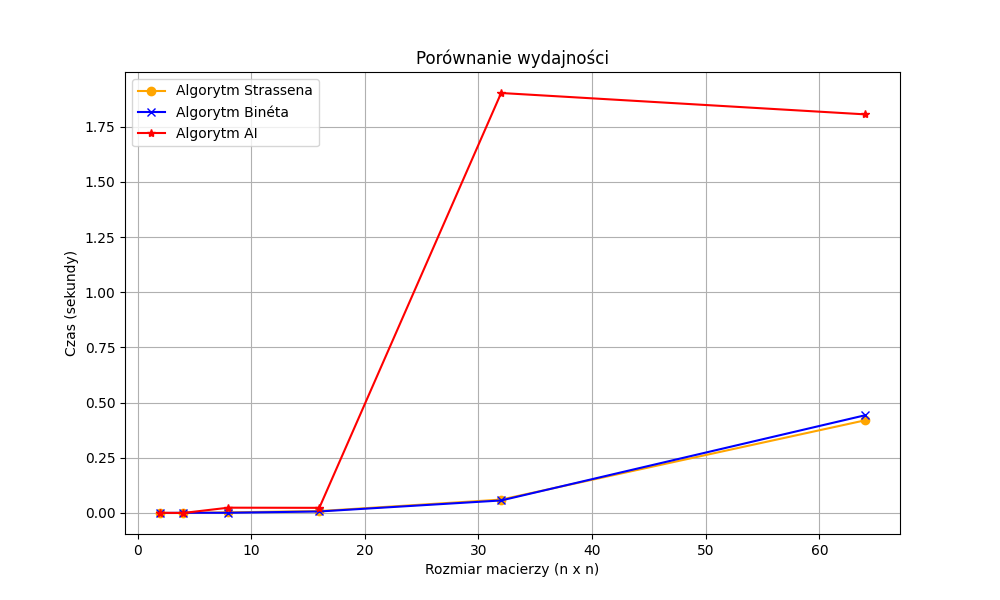
\includegraphics[width=0.9\linewidth]{czas_dzialania1.png}
        \caption{Porównanie czasu działania.}
    \end{figure}
    Czas działania algorytmów dla $n=2^m$, gdzie
    \[
        m \in [2, 64]
    \]
    \begin{figure}[H]
        \centering
        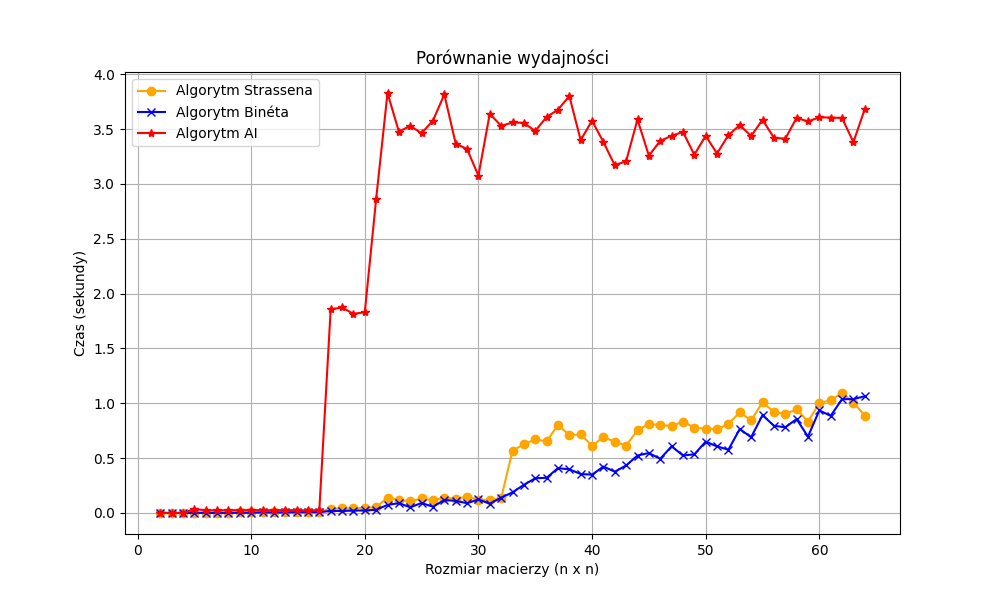
\includegraphics[width=0.9\linewidth]{czas_dzialania2.png}
        \caption{Porównanie czasu działania.}
    \end{figure}

    \subsection{Liczba operacji zmienno-przecinkowych}
    Liczba operacji zmienno-przecinkowych wykonanych podczas
    działania algorytmów dla $n=2^m$, gdzie
    \[
        m \in \{2,4,8,16,32,64\}
    \]
    \begin{figure}[H]
        \centering
        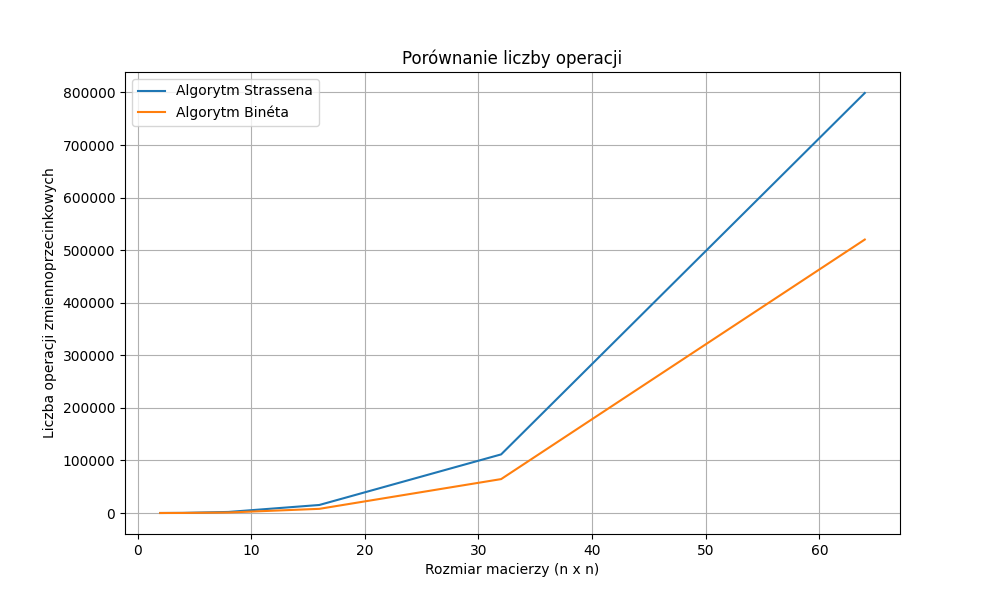
\includegraphics[width=0.9\linewidth]{liczba_operacji1.png}
        \caption{Porównanie liczby operacji zmienno-przecinkowych.}
    \end{figure}
    Liczba operacji zmienno-przecinkowych wykonanych podczas
    działania algorytmów dla $n=2^m$, gdzie
    \[
        m \in [2, 64]
    \]
    \begin{figure}[H]
        \centering
        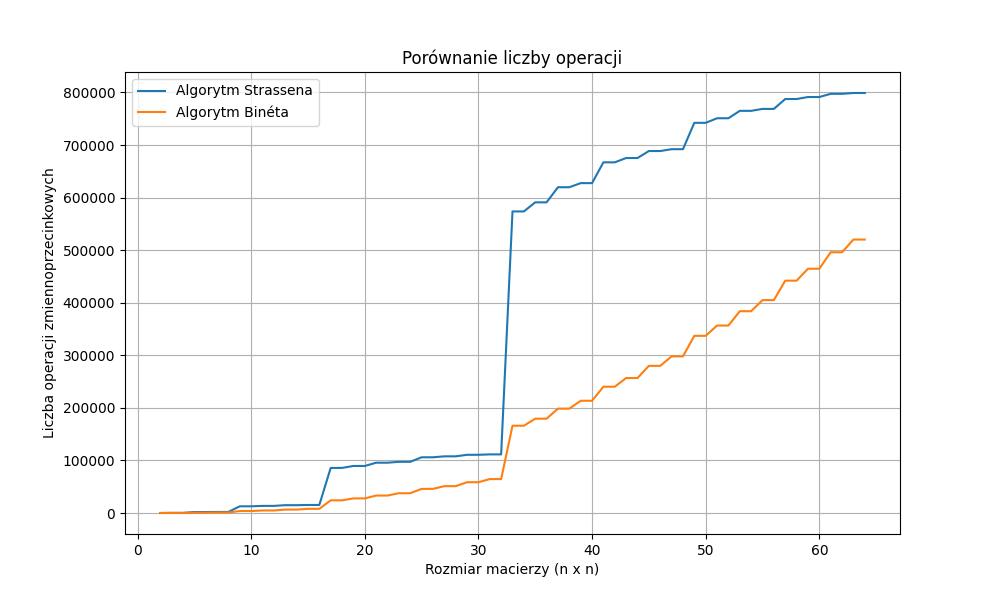
\includegraphics[width=0.9\linewidth]{liczba_operacji2.png}
        \caption{Porównanie liczby operacji zmienno-przecinkowych.}
    \end{figure}

    \section{Oszacowanie złożoności obliczeniowej}
    Dla każdego algorytmu zmierzony został czas obliczeń dla
    następujących wielkości macierzy:
    \[
        n \in \{2,4,8,16,32,64,128\}
    \]
    oraz dopasowana krzywa złożoności obliczeniowej.
    
    \subsection{Algorytm Binét'a}
    Dopasowana krzywa:
    \[
        y=2*10^{-6}*x^3
    \]
    Zatem złożoność wynosi
    \[
        O(n) \approx n^3
    \]
    \begin{figure}[H]
        \centering
        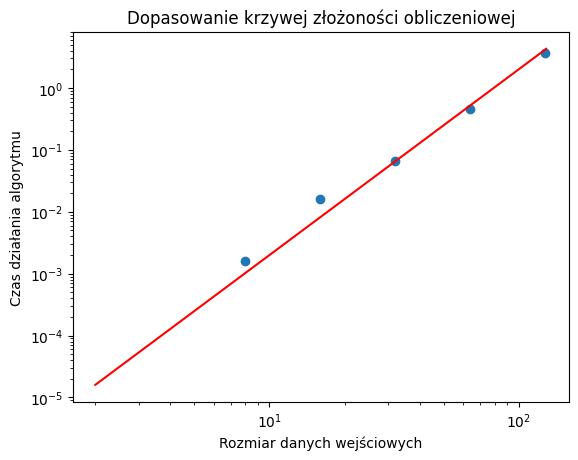
\includegraphics[width=0.8\linewidth]{zlozonosc_binet.png}
        \caption{Krzywa dopasowana w skali logarytmicznej dla
            algorytmu Binét'a.}
    \end{figure}

    \subsection{Algorytm Strassena}
    Dopasowana krzywa:
    \[
        y=2*10^{-5}*x^{2.5}
    \]
    Zatem złożoność wynosi
    \[
        O(n) \approx n^{2.5}
    \]
    \begin{figure}[H]
        \centering
        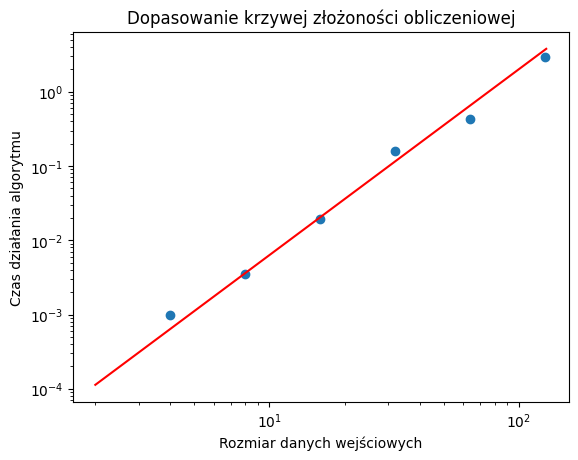
\includegraphics[width=0.8\linewidth]{zlozonosc_strassen.png}
        \caption{Krzywa dopasowana w skali logarytmicznej dla
            algorytmu Strassena.}
    \end{figure}

    \subsection{Algorytm AI}
    Dopasowana krzywa:
    \[
        y=1.8*10^{-5}*x^3
    \]
    Zatem złożoność wynosi
    \[
        O(n) \approx n^3
    \]
    \begin{figure}[H]
        \centering
        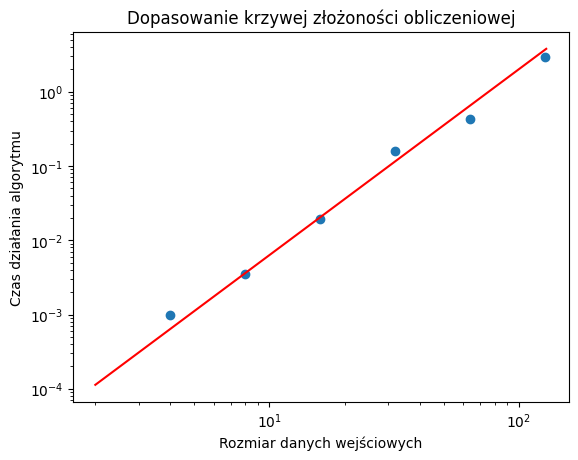
\includegraphics[width=0.8\linewidth]{zlozonosc_strassen.png}
        \caption{Krzywa dopasowana w skali logarytmicznej dla
            algorytmu AI.}
    \end{figure}

    \section{Porównanie obliczeń ze srodowiskiem Matlab}
    Na wejściu mamy macierz $A$ i $B$. Wartości wewnątrz macierzy:
    \begin{figure}[H]
        \centering
        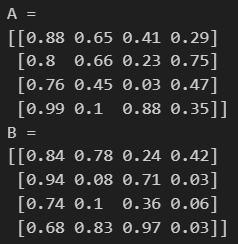
\includegraphics[width=0.4\linewidth]{porownanie_wejscie.png}
        \caption{Wartości macierzy $A$ i $B$.}
    \end{figure}

    \subsection*{}
    Wyniki mnożenia macierzy uzyskane za pomocą każdego z zaimplementowanych
    algorytmów:
    \begin{figure}[H]
        \centering
        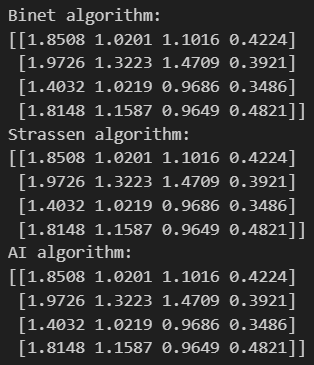
\includegraphics[width=0.5\linewidth]{porownanie_wyjscie_alg.png}
        \caption{Wyniki algorytmów.}
    \end{figure}

    \subsection*{}
    Wyniki mnożenia macierzy obliczone za pomocą środowiska Matlab:
    \begin{figure}[H]
        \centering
        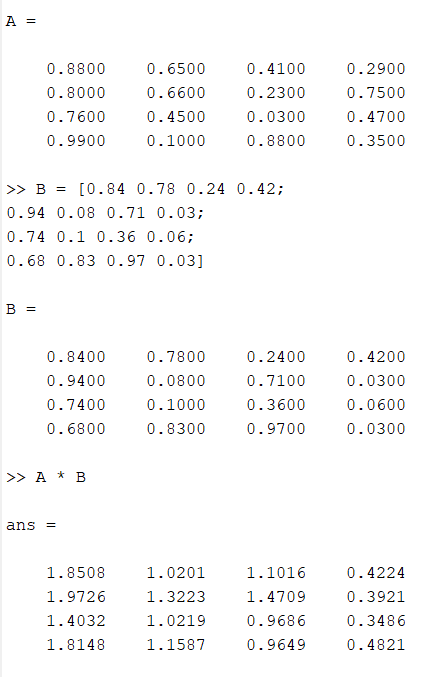
\includegraphics[width=0.6\linewidth]{porownanie_wyjscie_matlab.png}
        \caption{Wyniki środowiska Matlab.}
    \end{figure}

    \subsection*{}
    Wyniki uzyskane za pomocją zaimplementowanych algorytmów są identyczne
    z wynikami otrzymanymi ze środowiska Matlab. Można wnioskować, że
    przedstawione algorytmy działają poprawnie.
\end{document}
